\documentclass[a4paper,12pt, projekat]{etf}
\usepackage[intlimits]{amsmath} 
\usepackage{amsmath, amsfonts, amssymb, graphicx}
\usepackage[section]{placeins}

\usepackage[serbian]{babel} 
\usepackage[T1]{fontenc}
\usepackage[utf8]{inputenc}
\addto\captionsserbian{% r
  \renewcommand{\bibname}%
    {Literatura}%
}

\title{Semaforizovana raskrsnica}
\author{Marko Ljubisavljević i Luka Orlandić}
\indeks{2014/0620 i 2015/0390}
\date{avgust 2018.}
\mentor{prof.~dr Milan Bjelica}
\predmet{Principi modernih telekomunikacija}


\begin{document}
    \maketitle
    \begin{abstract}
    	U okviru predmeta Principi modernih telekomunikacija (u daljem tekstu PMT) realizovali smo Semaforizovanu raskrsnicu koju je moguće konfigurisati iz Grafičkog korisničkog interfejsa (GUI-a). Projekat predstavlja direktnu spregu hardware-a (\textit{kombinacionih prekidačnkih mreža}) i software-a (\textit{programiranje i sinhronizacija raskrsnice u programskim jezicima C i Python}). Na kraju kao rezultat projekta, raskrsnica sa semaforima je sinhronizovana i spremna za korišćenje u realnom vremenu. 
    \end{abstract}
    \begin{keywords}
        Semafor, Raskrsnica, C, Python, UART
    \end{keywords}
   \tableofcontents
   \listoffigures
   % \listoftables
    
% Chapter: Uvod 
\chapter{Uvod}

% Section: Cilj projekta
\section{Cilj \& zamisao projekta}
Veoma je intuitivno odrediti cilj ovog projekta: Napraviti jednostavnu semaforizovanu raskrsnicu sa semaforima za automobile i pešake koji su međusobno sinhronizovani. Prilikom sinhronizacije potrebno je voditi računa o praktičnim problemima (npr. trepćuće zeleno koje se pali onda kada pravac kojim se kreću automobili treba da izgubi mogućnost prolaska) i mnogim drugim.

% Section: Hardware
\section{Hardware}
Za paljenje svetala na semaforima koristili smo mikrokontroler TI \textbf{MSP430G2553}. Dodatne elektronske komponente koje smo korisitili u realizaciji su kombinacione prekidačke mreže SN74LS04 (\textit{NOT gate}), SN74HCT139 (\textit{Dual 2-input Decoder}) i SN74HCT32 (\textit{OR gate}).

\begin{figure}[!htb]
\centering
\includegraphics[width=400px]{GVDesign/components.png}
\caption{\textit{Logička kola korišćena u izradi projekta.}}
\label{fig:logicgates}
\end{figure}

% Section: Software
\section{Software}
Logičko ''povezivanje'' semafora kao i paljenje svetala na njima koristi osnove jezika C i Python. Mikrokontroler je programiran u C-u (za njega je napravljen manji skup funkcija koji omogućava lakše korišćenje) a odlučivanje koje svetlo će na kom semaforu biti upaljeno - za to je odgovoran Python3.7. Komunikacija između mikrokontrolera i korisničkog računara se odvija putem \textit{USCI UART komunikacije}.

% CHAPTER: Projektni zadatak
\chapter{Projektni zadatak}
Kao što je već rečeno, potrebno je napraviti semaforizovanu raskrsnicu i osposobiti je da bude od praktičnog značaja. Rezultat izrade treba da bude jednostavna aplikacija koja omogućava korisniku upravljanje i naprednu sinhronizaciju na samoj raskrsnici.

\section{Semaforizovana raskrsnica}
Kao model raskrsnice koja je korišćena u ovom projektu uzeta je ona u kojoj se ukrštaju dva putna pravca po devedeset stepeni. Postoji ukupno 4 automobilska i 8 pešačkih semafora i to:
\begin{itemize}
  \item 2 x 2 semafora za automobile po jednom putnom pravcu
  \item 2 x 4 semafora za pešake po jednom putnom pravcu
\end{itemize}

\begin{figure}[!htb]
\centering
\includegraphics[width=240px, height=250px]{raskrsnica.png}
\caption{\textit{Šema raskrsnice korišćena u projektu.}}
\label{fig:intersectionschema}
\end{figure}


Semafori S1 i S2 su automobilski semafori koji prate odgovarajuće putne pravce. Pešački semafori koji su upareni uz njih su SP3 (\textit{Semaphore Passengers}) i SP4. U nastavku je data slika raskrsnice koja je korišćena u projektu.
\\
\\
\\
\\
\\
\\
\\


\section{Kombinaciona prekidačka mreža}
Sve komponente korišćene u ovom projektu su proizvedene od strane \textit{Texas Instruments}-a.

\subsection{Semafor za automobile}
Kako bi omogućili semaforu da svetli bilo je potrebno napraviti omanju prekidačku mrežu. U okviru jednog ciklusa rada semafora na njemu postoje 4 različite situacije, i to (predstavljeni binarnim vrednostima):
\begin{itemize}
  \item 00 - Crveno + Žuto
  \item 01 - Zeleno
  \item 10 - Žuto
  \item 11 - Crveno
\end{itemize}
Situacija kada na semaforu trepće žuto ili zeleno obrađena je softverski o čemu će biti reči u nastavku.\\
Kako postoje 4 kombinacije vrednosti potrebne da se opiše stanje semafora, dovoljan nam je bio dekoder \textit{\textbf{SN74HCT139} Dual 2-input Decoder}.
Izlazi dekodera daju invertovanu vrednost (\textit{active low}), što nam dodatno povećava kombinacionu šemu. Kako bi rešili ovaj problem dodali smo invertor \textbf{SN74LS04}.\\
Potrebno je odrediti u kojim situacijama se pali određeno svetlo.\\
Crveno svetlo se pali kada je aktivno:
\begin{itemize}
  \item 00 - Crveno + Žuto, \textbf{ili}
  \item 11 - Crveno
\end{itemize}
Žuto svetlo se pali kada je aktivno:
\begin{itemize}
  \item 00 - Crveno + Žuto, \textbf{ili}
  \item 10 - Žuto
\end{itemize}
Gornji prikaz situacija kada se pojavljuje određeno svetlo govori da nam je potrebno jedno OR logičko kolo. U našem projektu smo koristili \textit{\textbf{SN74HCT32} (Quad 2-input OR Gate)} kako bi povezali signalizaciju za žuto i crveno svetlo. Zeleno svetlo se pali samo u jednoj situaciji - kada je ulaz dekodera \textit{0b01} - pa izlaz invertora možemo direktno da povežemo na zelenu LE diodu na šemi.
\textbf{Enable bit} samog dekodera je aktivan kada je povezan na masu (\textit{active low}).

\subsection{Semafor za pešake}
Semafor za pešake je dosta jednostaviji za realizaciju. On ima samo dva stanja pa je potreban jedan dekoder čiji su ulazi tumačeni na sledeći način:
\begin{itemize}
  \item 0 - Crveno
  \item 1 - Zeleno
\end{itemize}
Kako izlazi dekodera daju invertovanu vrednost, potrebno je dodati samo jedan invertor i semafor je spreman za korišćenje. 

\subsection{Strukturne šeme}
U nastavku su date strukturne šeme semafora za automobile i za pešake. Treba računati da je potrebno naraviti još jedan primerak tih šema za semafore u suprotnom smeru.

\begin{figure}[!htb]
\centering
\includegraphics[width=400px]{GVDesign/schema1.png}
\begin{center}
\caption{\emph{Kombinaciona mreža za semafor za automobile.}}
\end{center}
\label{fig:comnetvehicles}
\end{figure}

\begin{figure}[!htb]
\centering
\includegraphics[width=400px]{GVDesign/schema2.png}
\begin{center}
\caption{\emph{Kombinaciona mreža za semafor za pešake.}}
\end{center}
\label{fig:comnetpassengers}
\end{figure}

\section{Programiranje mikrokontrolera}
Kada je završena izrada hardverskog dela projekta, potrebno je povezati mikrokontroler sa ulaznim pinovima dekoderima i tako osposobiti paljenje svetala na semaforima.

\subsection{Opcode}
Opcode predstavlja dvobajtnu ''instrukciju'' koja sadrži informaciju o tome koji semafor kako treba da radi. Format instrukcije je dat u vidu slike i definisan je na sledeći način:

\begin{figure}[htb]
\centering
\includegraphics[width=400px]{GVDesign/opcode.png}
\caption{\emph{Prikaz opcode-a koji će parsirati mikrokontroler.}}
\label{fig:opcodepreview}
\end{figure}

\hfill \break

S1, S2, SP3, SP4 predstavljaju semafore sa slike 2.1, a ES1, ES2, ESP3, ESP4 su enable biti semafora S1, S2, SP3 i SP4, respektivno. Indeks S1$_{H}$ govori da je to viši bit koji se vodi na ulaze dekodera.
 
\subsection{Raspored pinova}
\label{title:micro_scheduling}
Potrebno je izvršiti raspodelu i zauzimanje pinova na mikrokontroleru. U okviru njega postoje:
\begin{itemize}
  \item P1.0 - out
  \item P1.1 - UART reserved
  \item P1.2 - UART reserved
  \item P1.(3..7) - out
  \item P2.(0..3) - out
\end{itemize}
Ovo je spisak svih pinova koji su nam bili potrebni za realizaciju projekta. Način na koji smo koristili alokaciju je sledeći:

\begin{figure}[!htb]
\centering
\includegraphics[width=400px]{GVDesign/pin_scheduling.png}
\begin{center}
\caption{\emph{Prikaz rasporeda pinova na mikrokontroleru MSP430G2553 koji je povezan sa kombinacionom prekidačkom mrežom.}}
\end{center}
\label{figure:micro_scheduling}
\end{figure}
\hfill \break \break
Enable biti se šalju onako kako zaista želimo da upravljamo semaforima (0 - ugašen, 1 - upaljen) bez obzira na to što je enable bit aktivan kada je jednak nuli (\textit{active low}). Funkcija koja vodi računa o tome je \verb|_enable_semaphore()| (pogledati poglavlje \ref{title:functions}).

\subsection{Funkcije za lakši rad}
\label{title:functions}
Da bi se omogućio lakši rad sa mikrokontrolerom, osmislili smo set funkcija koje mogu da se koriste prilikom programiranja. Sada kada znamo kako su određeni biti raspoređeni, potrebno je samo da baratamo sa pročitanim binarnim vrednostima.\\
Delimične deklaracije funckija koje olakšavaju rad date su u nastavku:
\begin{enumerate}
\item \verb|_enable_semaphore( semID, enable )|
\item \verb|_get_enable_bit_position( semID )|
\item \verb|_set_bits_for_vehicles( action, hbitpos, lbitpos )|
\item \verb|_set_bits_for_passengers( action, bitpos )|
\item \verb|_change_lights( semID, action )|
\item \verb|_parse_rdx( second, first )|
\end{enumerate}

U okviru funkcije \verb|_enable_semaphore( semID, enable )| uključujemo / isključujemo određeni semafor na osnovu njegovog ID-a. Na kombinacionu šemu se pušta invertovana vrednost \textbf{\textit{enable}} zbog strukture dekodera SN74HCT139.\\

Funkcija \verb|_get_enable_bit_position( semID )| vraća aktivan onaj bit koji odgovara enable bitu u rasporedu bitova na mikrokontroleru (koji smo videli gore - slika 2.5). Na primer, ako se prosledi semID = S2, funkcija vraća 0x2, što odgovara poziciji bita 1 u portu 2. Radi još bolje preglednosti, \textit{svi enable biti su izmešteni na port 2}.\\

Funkcija \verb|_set_bits_for_vehicles( action, hbitpos, lbitpos )| na osnovu akcije (npr. \textit{action = R (\textit{red})}) koja joj se prosledi, menja viši odnosno niži bit u portu P1 i samim tim prosleđuje onu kombinaciju koja je potrebna na ulaze dekodera.\\

Funckija \verb|_set_bits_for_passengers( action, bitpos )| radi isto što i gornja funkcija ali samo za pešačke semafore.\\

Funkcija \verb|_change_lights( semID, action )| menja svetlo na određenom semaforu sa zadatim ID-om na osnovu akcije koja može biti R (\textit{red}), Y (\textit{yellow}), RY (\textit{redyellow}), G (\textit{green}).\\

Funkcija \verb|_parse_rdx( second, first )| se poziva u UART prekidnoj rutini i služi da parsira prvi i drugi bajt dobijen prilikom transporta. Onog momenta kad se prime dve vrednosti, poziva se ova funkcija koja pali određena svetla na semaforima. Prvi i drugi bajt predstavljaju \textit{opcode}. \textbf{Napomena}: Parametri su pomereni zbog logičkog rasporeda bita - od najvišeg (sa leve strane) do najnižeg (sa desne strane).

\subsection{UART}
Komunikacija računara i mikrokontrolera MSP430G2553 se odvija preko \textit{USCI UART}-a. Pinovi koji su tada zauzeti su P1.1 i P1.2. Mikrokontroler postavlja prekidnu rutinu u kojoj može da pročita 8-bitni registar \textbf{UCA0RXBUF} koji predstavlja bafer u koji se smešta vrednost prenešena sa računara. Kratki insert koda u C-u ove prekidne rutine izgleda vrlo jednostavno:
\\
\\
\\
\\
\\

\begin{verbatim}
code[ received++ ] = UCA0RXBUF;
if ( received == 2 )
{
   _parse_rdx( code[1], code[0] );
   received = 0;
}
\end{verbatim}
Kao što se može primetiti, sa računara se prvo šalje prvi bajt, a potom odma iza njega drugi. Brojač podataka se resetuje vrlo jednostavno onda kada se kružni bafer za podatke \verb|char code[2]| napuni. Tada se i parsiraju bajtovi i pale određena svetla na semaforima.

\section{Sinhronizacija semafora}
Kada je osposobljavanje mikrokontrolera za efikasno korišćenje gotovo, ostaje da se napravi program (aplikacija) koja će da vodi računa o \textbf{sinhronizaciji semafora}. Osnovna zamisao jeste da jedan semafor putnog pravca drži crveno dok drugi napravi svoj puni ''zeleni'' ciklus. Iako korisnik ima puno pravo da menja trajanje svakog svetla na semaforu, automatsko računanje trajanja vremena garantuje da će semafori biti sinhronizovani. Pomoću programskog jezika \textit{Python} i \textit{QtDesigner}-a bili smo spremni da počnemo izradu aplikacije.

\subsection{Niz naredbi}
Kada korisnik unese dužinu intervala koji želi da primeni na raskrsnicu, kreiraju se nizovi sa elemenatima čije vrednosti mogu biti jednake \verb|R, RY, G, BG|. U ovom trenutku uvodimo novu vrednost koju semafor može da ima, vrednost \textit{BG} koja u ovom slučaju označava trepćuće zeleno (engl. \textit{blinking green}). Tačnije, \textbf{svaki element niza predstavlja jedan sekund na semaforu}. Na primer, ukoliko je niz \verb|sem1 = [R, R, R, RY, G, G, G, G, ...]| to znači da na semaforu 1 gori 3 sekunde crveno svetlo. Svake sekunde se preko UART-a šalju komande mikrokontroleru. Kada se iscrpi ceo niz, ciklus se završio što znači da ponovo krećemo od početka da brojimo. Tako obezbeđujemo (teorijski) beskonačno dugačku sekvencu rada semafora na raskrsnici.

\subsection{Thread}
\label{title:Thread}
Glavni paket koji smo koristili u izradi sinhronizacije semafora jeste zapravo \textit{Thread} paket. Pomoću njega smo vrlo jednostavno pravili niti koje vode računa o sinhronizaciji. Napravili smo:
\begin{enumerate}
\item \textbf{regular\_timer} thread
\item \textbf{fast\_timer} thread
\item \textbf{transition} thread
\item \textbf{yellow} thread
\end{enumerate}
Komunikacija kao i sinhronizacija \textbf{između niti} se odvijala upotrebom \textit{sinhronizacione primitive \textbf{Semaphore}}. Ova klasa ima dve metode: \textbf{acquire} - ekvivalent \textit{Semaphore.wait()} i \textbf{release} - ekvivalent \textit{Semaphore.signal()}.\\

Set funkcija pisanih u programskom jeziku \textit{Python} treba da pokupi stanja svih semafora u \verb|regular_timer| niti i da od njih napravi opcode koji će biti poslat mikrokontroleru (slika \ref{fig:opcodepreview}).\\

Nit \verb|fast_timer| se koristi onda kada neki od semafora ima naredbu trepćućeg zelenog. Tada se \verb|regular_timer| zablokira i u rad pušta nit \verb|fast_timer| čiji je sleep period skoro trostruko manji od \verb|regular_timer|-a. To znači da se kao efekat dobija da se svetla brže pale/gase tj. da blinkaju.\\

Nit \verb|yellow| je nit koja naizmenično pali žuto svetlo na svim semaforima za vozila (engl. \textit{toggle}). Rad ove niti označava da semafori nisu u funkciji.\\

Nit \verb|transition| se koristi u tranzicionom periodu, onda kada je korisnik konfigurisao semafore i pustio ih u pogon. Tada se aktivira ova nit koja par puta upali žuta svetla (blinka žuto svetlo) a potom zadrži žuto svetlo na semaforu dve sekunde. Potom se ova nit zablokira i u rad ponovo pušta nit \verb|regulat_timer| koja ponovo uzima naredbe za svaki semafor na raskrsnici. Ova pogodnost je dodata isključivo da bi se poboljašalo korisničko iskustvo.

\subsection{Serial}
U okviru paketa Serial smo koristili osnovne mogućnosti, kao što su otvaranje komunikacije sa uređajem (\textit{serial.open()}), slanje podataka na serijski port (\textit{serial.send()}) i na kraju gašenje konekcije (\textit{serial.close()}).\\
\\

\section{Izgled projekta}
U nastavku prilažemo fotografije gotovog projekta:

\begin{figure}[!htb]
\centering
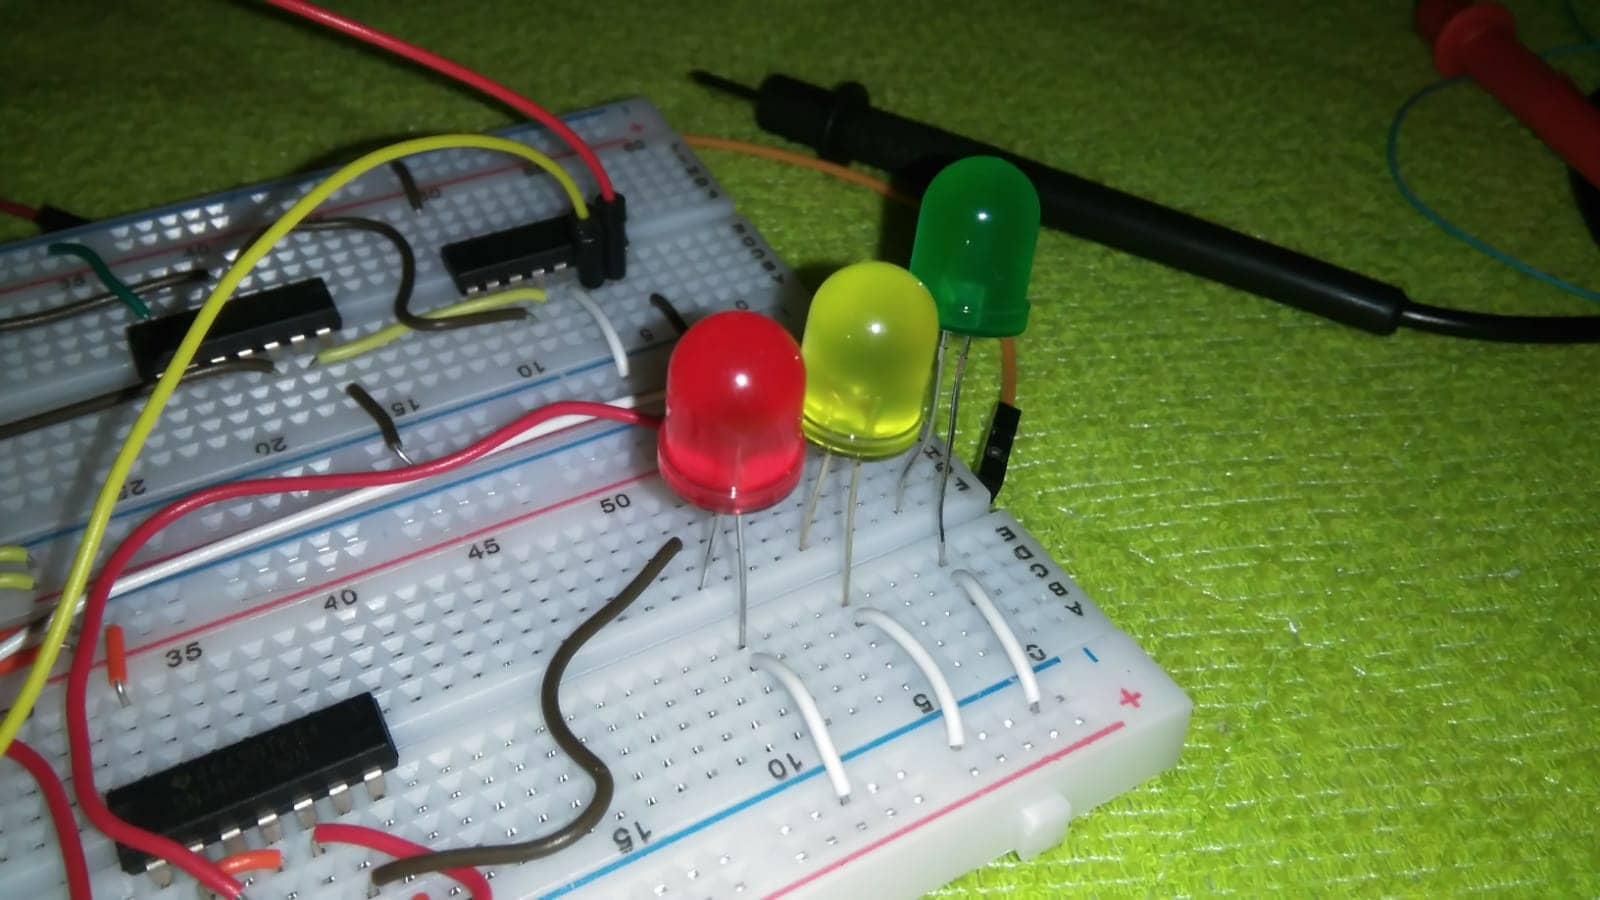
\includegraphics[width=400px]{images/s1.jpg}
\caption{\emph{Prikaz dela kombinacione prekidačke mreže za semafor za pešake.}}
\label{fig:im1}
\end{figure}

\begin{figure}[!htb]
\centering
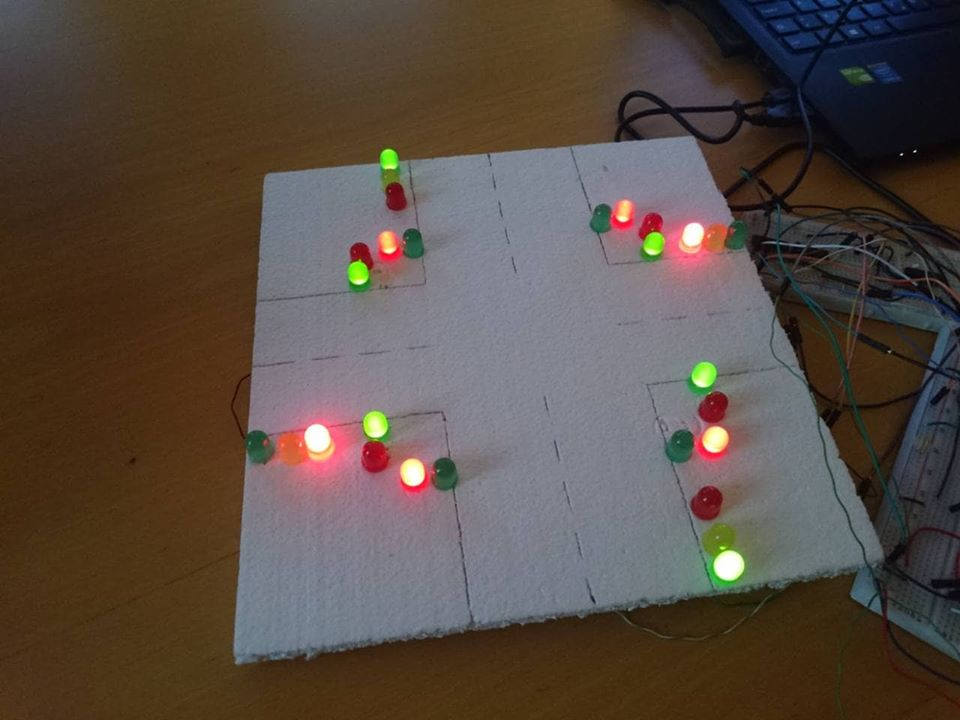
\includegraphics[width=400px]{images/s3.jpg}
\caption{\emph{Prikaz semaforizovane raskrsnice (detalj).}}
\label{fig:im2}
\end{figure}

\begin{figure}[!htb]
\centering
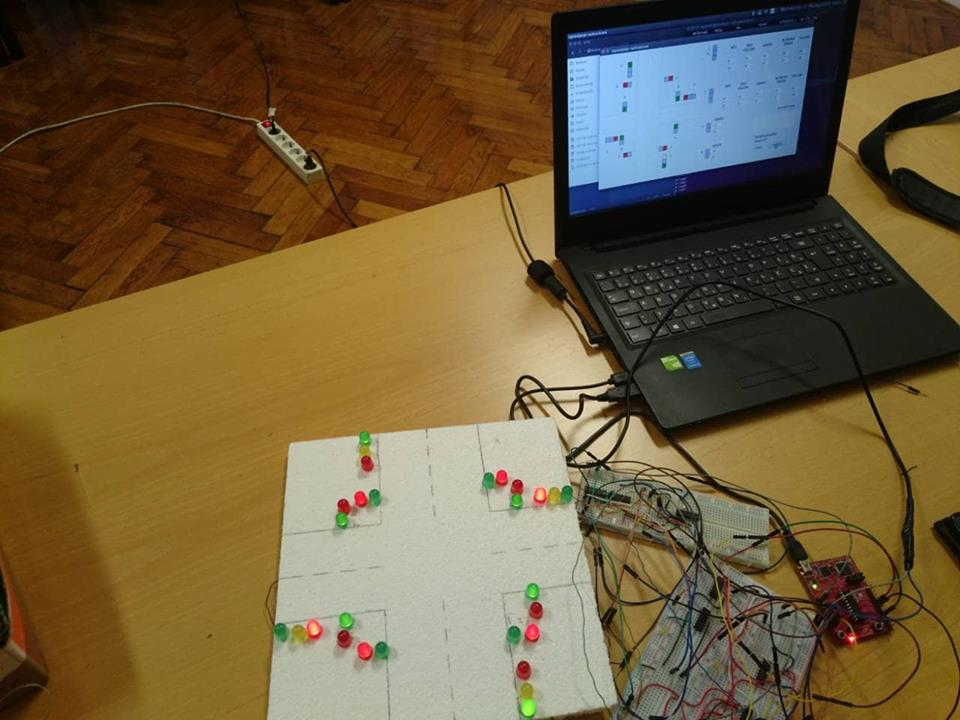
\includegraphics[width=400px]{images/s4.jpg}
\caption{\emph{Prikaz semaforizovane raskrsnice.}}
\label{fig:im3}
\end{figure}

\begin{figure}[!htb]
\centering
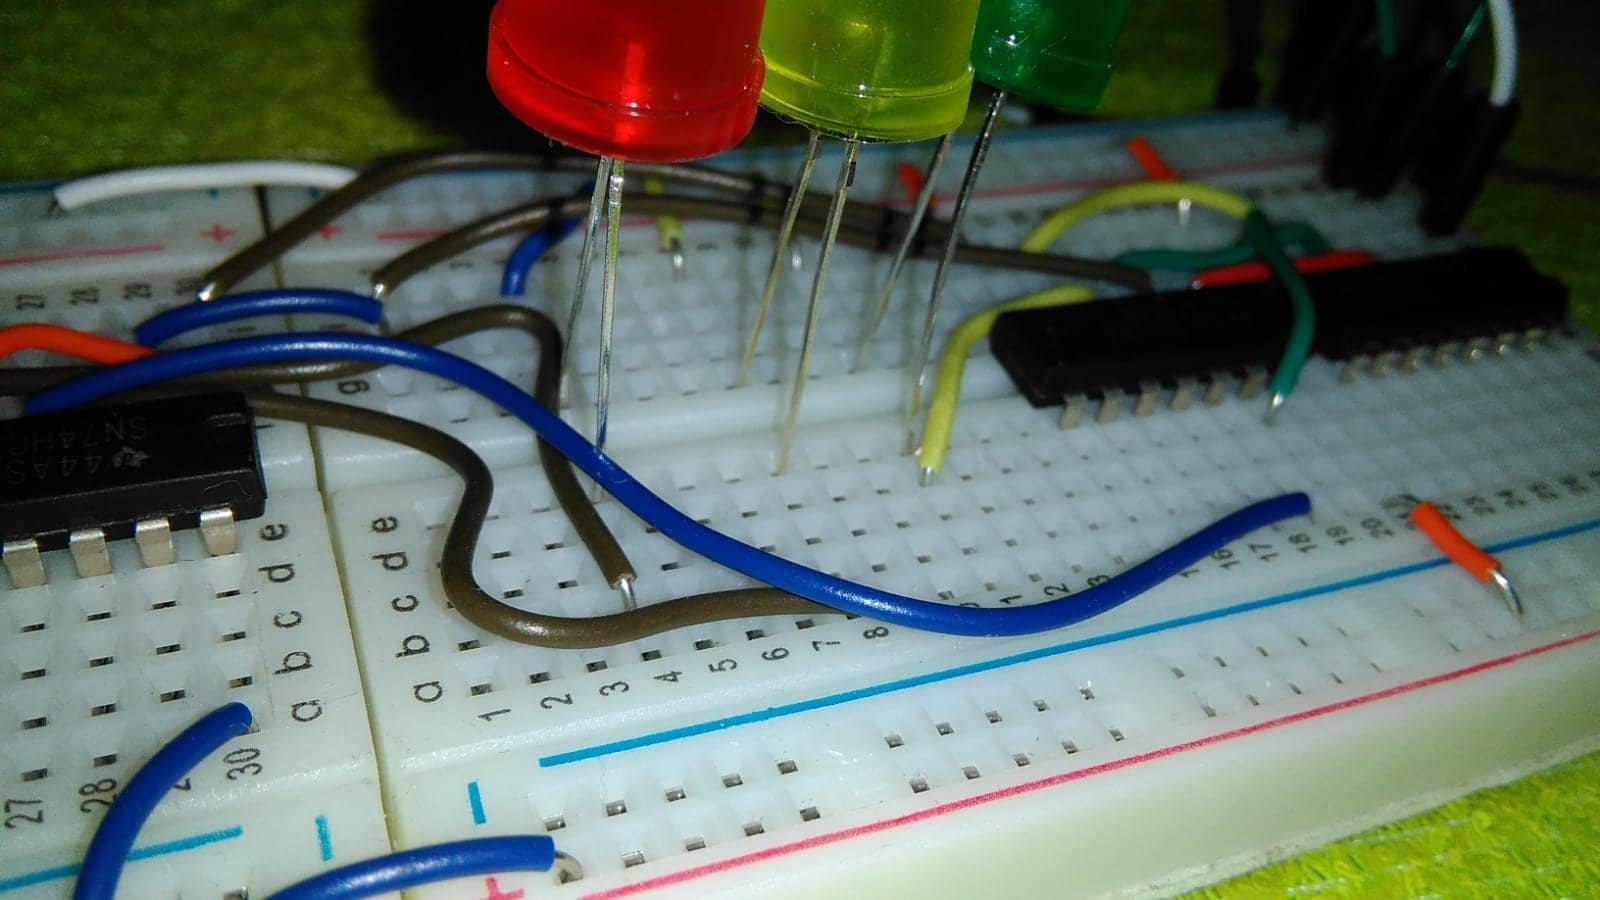
\includegraphics[width=400px]{images/s5.jpg}
\caption{\emph{Detalj kombinacione prekidačke mreže.}}
\label{fig:im3}
\end{figure}


% CHAPTER: Korisnička aplikacija
\chapter{Korisnička aplikacija}
Svaki korisnik računara voli da vizuelno ima pregled onoga što želi da uradi. Ako to pak nije slučaj, korisnik najčešće ne zna gde treba da klikne ili šta treba da uradi na računaru da bi postigao željeni cilj. Poznavajući želje samog korisnika, a istovremeno u skladu sa projektnim zadatkom, napravili smo aplikaciju upotrebom \textit{QtDesigner}-a i potom pokrenuli aplikaciju u \textit{Python}-u.

\section{\textit{GUI} dijagnostika}
U okviru GUI dijagnostike, korisniku je omogućeno da proizvoljno postavi vreme (u sekundama) za sve kombinacije svetala: \textit{Crveno}, \textit{Crveno + Žuto}, \textit{Zeleno}, \textit{Trepćuće zeleno}, \textit{Žuto}. Nakon uspešno popunjene vremenske linije prvog semafora, klikom na dugme ''\textit{Autofill fields}'', aplikacija proračunava najefikasniji opseg vrednosti za semafore, praveći semafore sinhronizovanim. Korisnik sam posle toga može da menja vrednosti na semaforu, a ukoliko naruši sinhronizovanost, program mu neće dozvoliti da nastavi dalje. Izgled aplikacije je dat u nastavku.

\begin{figure}[htb]
\centering
\includegraphics[width=400px]{gui.png}
\caption{\emph{Prikaz korisničke aplikacije.}}
\label{fig:guipreview}
\end{figure}


\section{Dodatne opcije}
U okviru dodatnih opcija, korisnik može da onesposobi (engl. \textbf{disable}) semafore i samim upali trepćuće žuto na njima. Ukoliko pak poželi da ponovo upali semafore, cela raskrsnica će proći kroz \textit{period tranzicije} (pogledati odeljak \ref{title:Thread} na strani \pageref{title:Thread}) i nakon 3-4 sekunde će se uspostaviti aktivno stanje semafora. Korisnik može i da potpuno ugasi raskrsnicu čime će svi semafori biti isključeni.

\section{Aplikacija ''u akciji''}
Kada se pravilno unesu vrednosti, rad aplikacije izgleda na sledeći način:

\begin{figure}[htb]
\centering
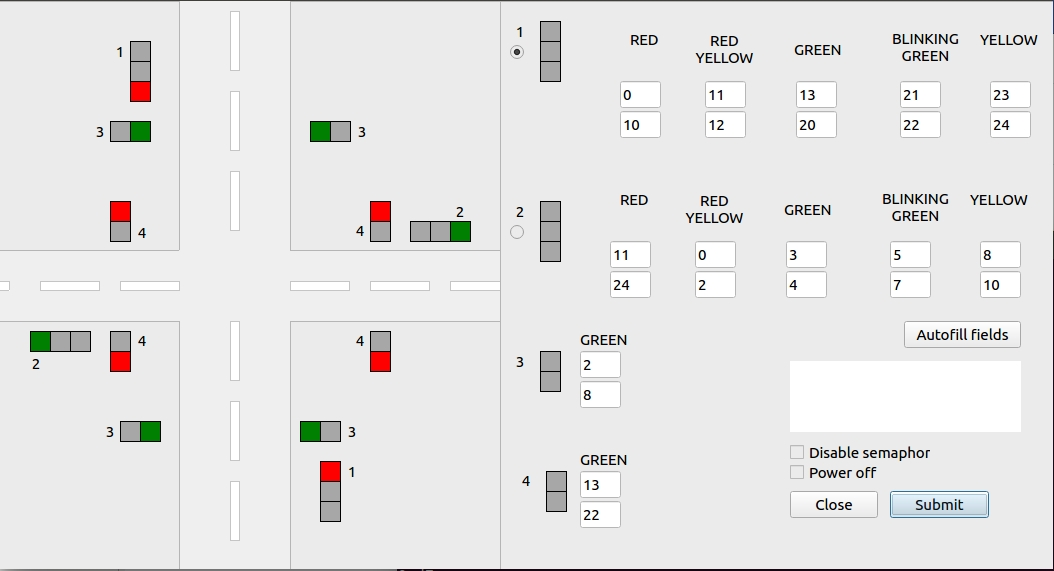
\includegraphics[width=400px]{images/s8.jpg}
\caption{\emph{Prikaz aplikacije kada je korisnik konfigurisao vrednosti.}}
\label{fig:im8}
\end{figure}

\begin{figure}[htb]
\centering
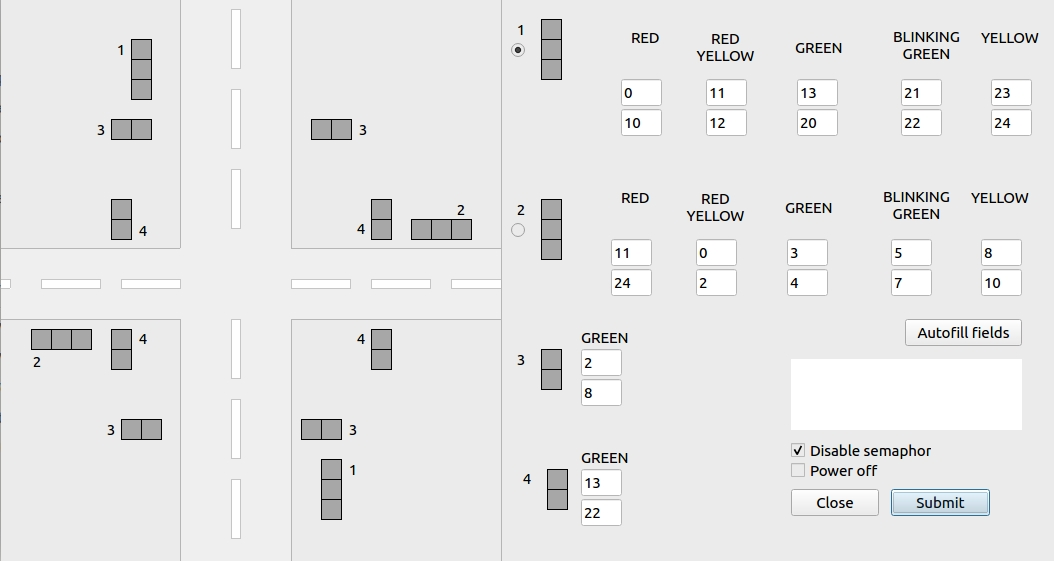
\includegraphics[width=400px]{images/s9.jpg}
\caption{\emph{Konfigurisanje vrednosti u aplikaciji.}}
\label{fig:im9}
\end{figure}

\begin{figure}[htb]
\centering
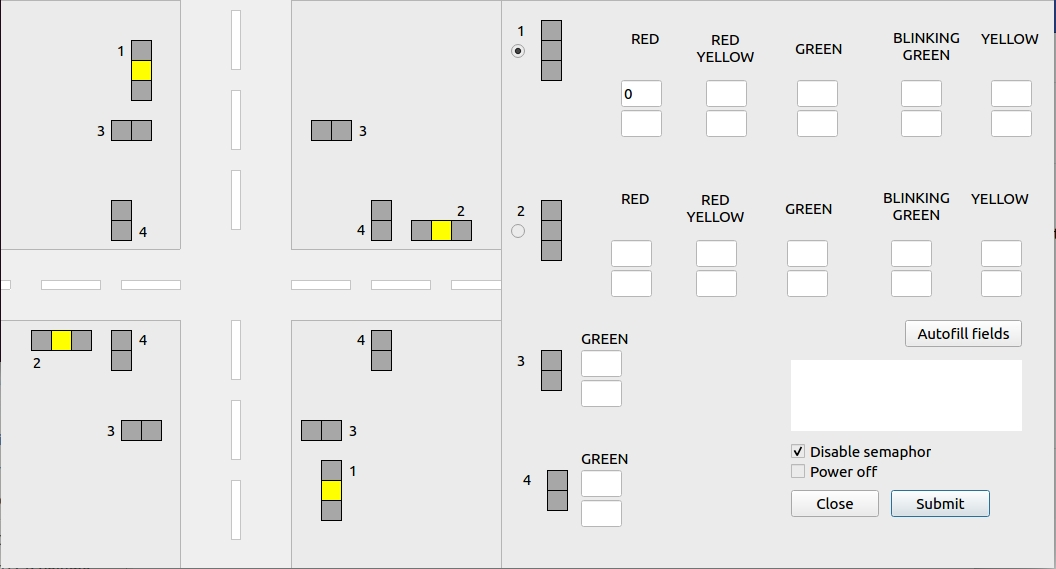
\includegraphics[width=400px]{images/s10.jpg}
\caption{\emph{Dodatna pogodnost: Svi semafori su onemogućeni.}}
\label{fig:im9}
\end{figure}

\chapter{Zaključak}
Celokupna izrada semaforizovane raskrsnice sa pravljenjem kombinacione prekidačke mreže proširuje stečeno znanje na predmetu PMT i na zanimljiv način približava studenta konkretnim problemima iz prakse.

\section{Način razmišljanja i algoritmi}
Iako deluje trivijalno, način razmišljanja je veoma bitan kod izrade projekta. Da li ćemo nešto zapisati sa tri bita ili samo sa jednim, dosta menja na planu dalje izrade projekta odnosno omogućava buduće modifikacije. Konkretno, u našem slučaju, uštedeli smo dosta pinova na mikrokontroleru koristeći dekodere i logička kola.\\
Što se tiče samih algoritama, pre svega mislimo na \textit{pseudokod}, odnosno skrećemo pažnju koliko je važno imati skicu onoga što je potrebno napraviti a potom to isto ''sprovesti u delo''.

\section{Prostor za modifikacije}
Kao i kod svakog drugog projekta, ostavljen je prostor za modifikacije koje je moguće naknadno implementirati u projektu. Kao jedna od dodatnih modifikacije bi bila recimo sinhronizacija ulice (sa od po dva semafora) koji bi trebalo da smanje gužvu na ulicama. Modifikacija se može dodatno napraviti sa dodavanjem uslovnog zelenog svetla na jednom ili sva četiri skretanja (što na terenu nije tako čest slučaj). Takođe, ono što je zanimljivo jeste da se mogu dodati tasteri za pešake kako bi mogli još brže da pređu ulicu i tako zatvore semafore pre vremena.
    
% Literatura
\begin{thebibliography}{10}
\addcontentsline{toc}{chapter}{Literatura}
\bibitem{lat} \emph{http://www.ti.com/lit/ds/symlink/msp430g2553.pdf}, 16.08.2018.
\bibitem{lat2} \emph{https://docs.python.org/3.4/library/asyncio-sync.html\#semaphores}, 16.08.2018.
\bibitem{lat3} \emph{https://pyserial.readthedocs.io/en/latest/pyserial.html}, 16.08.2018.
\bibitem{lat4} \emph{http://www.ti.com/lit/ds/symlink/sn54ls04-sp.pdf}, 16.08.2018.
\bibitem{lat5} \emph{http://www.ti.com/lit/ds/symlink/sn54ls04-sp.pdf}, 16.08.2018.
\bibitem{lat6} \emph{http://www.ti.com/lit/ds/symlink/sn54ls139a-sp.pdf}, 16.08.2018.
\end{thebibliography}

\end{document}
